Perceptron model was proposed by Frank Rosenblatt in 1943 to design the model to 
mimic the human brain \citep{939589}. Perceptron model or the single-layered feed forwards network 
networks take the vectors of inputs and multiply with a randomly 
initialized weights and add random bias to network and process the information by providing data to the
activation function to process the information \citep{AGATONOVICKUSTRIN2000717}.

\begin{figure}[!htp]
    \centering
    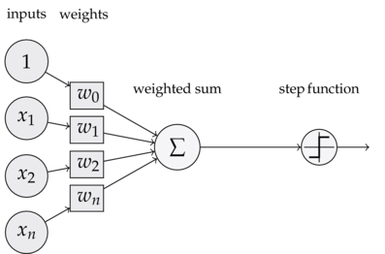
\includegraphics[width=0.6\textwidth]{Images/p_model.png} 
    \caption{Perceptron Model}
    \label{figure:perceptron}
\end{figure}
The figure \ref{figure:perceptron} represents the simple perceptron model which consists of inputs x and weights w 
for which the weighted sum of multiplication result of 
inputs and weights will be passed to the step activation function.

\subsection{Mathematical Representation }
\vspace{3mm}
{The equation below represents the preceptron model mentioned above in Mathematical notations.}
\begin{equation}
    \begin{split}
        y = \Big[\sigma(\sum_{k=0}^n x_k.w_k + b_k)\Big] \\
    \end{split}
\end{equation}

     {
        In, equation above ${\sigma = Activation function}$, x and w represents the inputs provided 
        and weights vectors in the network respectively. Furthermore, the symbol b represents the bias in the equation, 
        during the optimization of the network weights and bias are adjusted accordingly to improve the prediction. There are various activation functions ${\sigma}$ such as step function sigmoid, 
        relu, leaky relu and others that can be applied based on the requirements of the model prediction.
    }